\section{Standard 3: Full Methods and Data Transparency}


\begin{figure*}[t!]
    \centering
    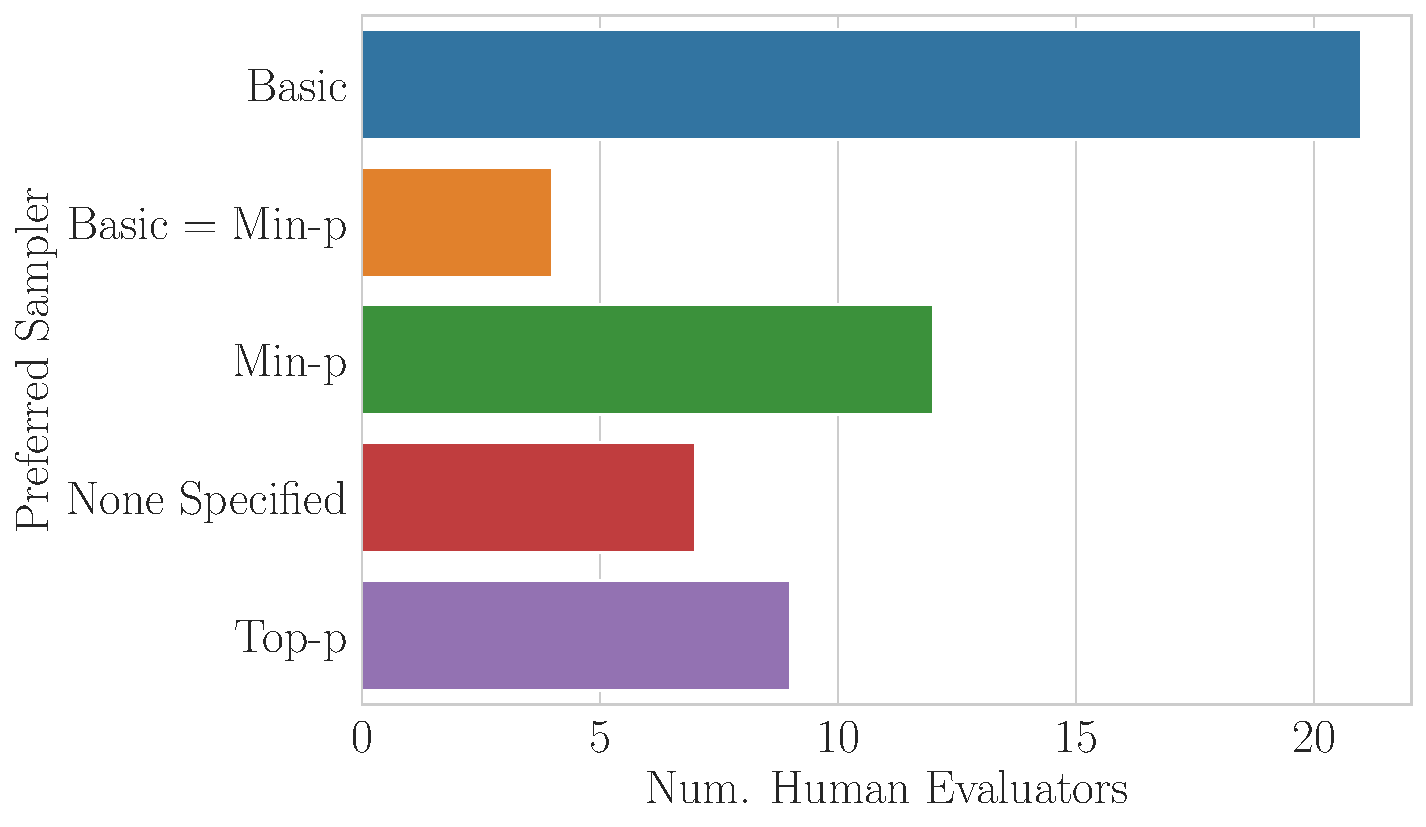
\includegraphics[width=0.7\linewidth]{figures/human_evals/attentive_human_annotators_preferred_samplers.pdf}
    \caption{\textbf{Manual Annotation of Human Evaluators' Qualitative Responses Fail to Support Claim that \texttt{Min-P} Was the Preferred Sampler.} We manually annotated responses from human annotators regarding their preferred sampler(s) at the end of the original paper's study. The responses suggest \texttt{min-p} was not the most preferred sampler. Example responses are provided in Appendix.~\ref{app:sec:human_qual_responses}.}
    \label{fig:attentive_human_annotators_preferred_samplers}
\end{figure*}

\paragraph{Human Evaluators’ Scores Were Omitted}
\label{sec:human_evals:subsec:omitted_data}

Section 6 of \citet{nguyen2024minp} states human participants evaluated \texttt{min-p} against a single sampler: \texttt{top-p}.
Multiple versions of manuscripts, including the \href{https://arxiv.org/abs/2407.01082v2}{Oct 2024 Arxiv manuscript} and \href{https://openreview.net/notes/edits/attachment?id=SR6ORZeBAn&name=pdf}{ICLR OpenReview manuscript}, repeatedly state that \texttt{min-p} and \texttt{top-p} were considered, and their Table 4 presents results only for these.
However, when examining the \href{https://github.com/menhguin/minp_paper/blob/main/min_p%20user%20preference%20study%20v2.0%20(Responses)%20-%20Form%20responses%201%20(1)%20(2).csv}{paper's data}, we discovered that scores for a second baseline sampler (\texttt{basic} sampling) were excluded from the methodology, the analysis and the results without mention or explanation. 
We \href{https://github.com/menhguin/minp_paper/issues/4}{publicly confirmed with the authors}.
These omitted scores comprised $1/3^{\text{rd}}$ of the total collected scores.
After we raised the issue, the omitted data were added to the \href{https://openreview.net/notes/edits/attachment?id=oQLYV9wuaa&name=pdf}{Camera Ready's Table 4}, but the methodology, the results and the conclusions have not been correspondingly updated.
As we showed in the previous section, the omitted data reveal that human evaluators actually preferred the baseline sampler over \texttt{min-p}.



\paragraph{LLM-As-A-Judge Evaluations Were Under-Specified and Indirect}

We next turned to the original paper's LLM-as-a-Judge evaluations \citep{zheng2023judging}, specifically AlpacaEval creative writing evaluations \citep{dubois2023alpacafarm}.
LLM-as-a-judge approaches have gained prominence as a scalable alternative to human evaluations, allowing researchers to assess model outputs across more prompts and conditions than would be feasible with human annotators alone.



% In the \href{https://arxiv.org/abs/2407.01082v2}{Oct 2024 Arxiv manuscript} and \href{https://openreview.net/notes/edits/attachment?id=SR6ORZeBAn&name=pdf}{ICLR OpenReview manuscript},
The methodology in the manuscript was under-specified in several ways: There is no mention which model(s) were sampled from, which model(s) served as the judge(s), or how hyperparameters were chosen or swept.
Additionally, there is no description of uncertainty for reported win rates, meaning win rates may be indistinguishable from chance (50.00\%).
Furthermore, the experiment seems designed in a manner that introduces a confounder. As context, AlpacaEval reports win rates between pairwise comparisons.
Instead of directly comparing \texttt{min-p} against other samplers, the authors compared each sampler against a common fixed sampler: \texttt{basic}$(\tau=1.0)$.
This comparison strategy is indirect; comparing directly against \texttt{min-p} would offer a clearer assessment of its superiority while using the same number of comparisons.
The experimental design is additionally concerning because LLM-judge preferences are not transitive, as shown by recent research \citep{xu2025investigatingnontransitivityllmasajudge}; that is, if sampler A beats sampler B, and sampler B beats sampler C, it does not necessarily follow that sampler A beats sampler C.
Therefore, comparing all methods to \texttt{basic}$(\tau=1.0)$ provides no reliable inference about \texttt{min-p}’s performance relative to \texttt{top-p} or \texttt{basic} at other temperatures. These under-specified aspects of the methodology and the indirect experimental design hinder interpretation and reproduction of the results.
